\documentclass[11pt]{article}
\usepackage[margin=1in]{geometry}
\usepackage{booktabs,graphicx,amsmath,hyperref,enumitem,array}
\setlist{itemsep=2pt,topsep=3pt}
\hypersetup{colorlinks,linkcolor=black,urlcolor=blue}

\title{\textbf{Experimental Design Report}\\[4pt]\large Knowledge Distillation for Backward Compatibility:\\
Moving a Modern-Operator Model onto a Legacy Op Set}
\author{Guancheng (Austin) Chen}
\date{Code and raw results: \url{https://github.com/austinchennn/kd-legacy-hw}}

\begin{document}\sloppy
\maketitle

\noindent\textbf{Scope of this document.} A self-contained description of the experimental design:
the research question, data, models, experimental groups, evaluation protocol, results
(reported as obtained, including negative results), limitations, and where the conclusion stands.

\tableofcontents

\section{Research Question and Scope}
\textbf{Overall goal.} New ML models increasingly depend on operators (GELU, LayerNorm, softmax attention)
that older AI accelerators and edge DSPs, built around INT8 convolution pipelines, cannot execute natively.
The question: \emph{can a model restricted to a legacy operator set, trained with knowledge distillation (KD)
from a modern-operator model, reproduce that model's behaviour at acceptable accuracy and latency?}

\medskip\noindent\textbf{Sub-questions.}
\begin{enumerate}[label=Q\arabic*.]
  \item What does the op-set restriction cost in accuracy, size and latency?
  \item Does logit KD make the legacy student \emph{behave more like} the teacher (prediction agreement), beyond accuracy?
  \item Does INT8 post-training quantization, the usual legacy-hardware format, preserve the result?
\end{enumerate}

\noindent\textbf{Explicit scope limitation.}
\begin{center}\begin{tabular}{ll}\toprule
Dimension & Coverage of this study\\\midrule
Task / data & Image classification, CIFAR-10 only\\
Teacher & One small ViT trained from scratch (no pre-training)\\
Student & One fixed VGG-style CNN architecture\\
KD method & Vanilla logit KD (Hinton et al., 2015) only\\
``Legacy hardware'' & Emulated: op-set whitelist + INT8 PTQ + 1-thread CPU latency\\\bottomrule
\end{tabular}\end{center}
The conclusion is therefore stated as ``a feasibility study with an emulated legacy target'', not as a
claim about any specific accelerator.

\section{Dataset Design}
\begin{itemize}
  \item CIFAR-10: 50{,}000 train / 10{,}000 test, $32\times32$ RGB, 10 classes; standard per-channel normalization.
  \item Augmentation (train only): reflect-pad 4 + random $32\times32$ crop, horizontal flip ($p=0.5$),
        executed on-device. \emph{Implementation note:} the crop offset is sampled once per mini-batch
        (the flip is per-sample); this is weaker than per-sample cropping and applies identically to all groups.
  \item No validation split was carved out; no hyper-parameters were tuned on the test set
        (all settings were fixed before the runs; see \S\ref{sec:repro}).
  \item INT8 calibration: the first 2{,}048 training images.
\end{itemize}

\section{Model Design}
\begin{center}\begin{tabular}{p{2.1cm}p{6.3cm}p{5.6cm}}\toprule
 & Teacher (``new'' model) & Student (``legacy-compatible'')\\\midrule
Architecture & ViT: patch 4 (64 tokens), dim 256, depth 6, 8 heads, MLP ratio 2, mean-pool head &
VGG-style: $2\times$[Conv$3\times3$-BN-ReLU] per stage, widths 32/64/128, MaxPool, GAP, Linear\\
Params & 3.19M & 0.29M\\
Operators & GELU, LayerNorm, softmax attention (\emph{not} on legacy list) &
Conv, BN, ReLU, MaxPool, AvgPool, Linear (all on legacy list)\\
Deployment & FP32 & FP32 and INT8 (Conv-BN-ReLU fused, PTQ, qnnpack)\\\bottomrule
\end{tabular}\end{center}
The legacy operator whitelist is \texttt{models.LEGACY\_OPS}; compatibility is checked automatically over leaf modules.

\section{Experimental Groups}
\begin{center}\small\begin{tabular}{llp{7.6cm}ll}\toprule
Group & Model & Training signal & Epochs & Seeds\\\midrule
T & Teacher ViT & CE + label smoothing 0.1; AdamW $10^{-3}$, wd 0.05 & 100 & 1\\
S & Student, scratch & CE; SGD-Nesterov 0.05, mom 0.9, wd $5\!\times\!10^{-4}$ & 40 & 3\\
K & Student, KD & $0.9\,T^2\,\mathrm{KL}(p_t^{T}\,\|\,p_s^{T}) + 0.1\,\mathrm{CE}$, $T=4$; same optimizer as S & 40 & 3\\\bottomrule
\end{tabular}\end{center}
All groups: batch 256, One-Cycle LR (15\% warm-up). S and K differ \emph{only} in the loss (same seeds,
architecture, optimizer, schedule), so S is the control for K. Each student checkpoint is evaluated in FP32 and in INT8.

\section{Evaluation Metric System}
\begin{enumerate}
  \item \textbf{Accuracy}: top-1 test accuracy.
  \item \textbf{Behavioural compatibility}: agreement = fraction of test images where student and teacher predict the same class.
        Decomposed by teacher correctness: agreement on teacher-correct vs.\ teacher-wrong images.
  \item \textbf{Legacy-hardware cost}: unsupported-op count; parameters; serialized size;
        batch-1 latency on \textbf{one CPU thread} (median of 300 runs after 30 warm-up; Apple M4 Max).
  \item \textbf{Quantization robustness}: FP32 $\rightarrow$ INT8 change in accuracy and agreement.
\end{enumerate}
Seeds: mean $\pm$ sample std over 3 seeds.

\section{Results (reported as obtained)}
\subsection{Main table}
\begin{center}\begin{tabular}{lcccccc}\toprule
Model & Acc (\%) & Agree (\%) & Params & Size & Lat.\ (ms) & Unsupp.\ ops\\\midrule
T: ViT, FP32 & 85.67 & 100 & 3.19M & 12.8 MB & 1.48 & 3\\
S: scratch, FP32 & 89.86 $\pm$ 0.13 & 83.63 $\pm$ 0.16 & 0.29M & 1.17 MB & 0.49 & 0\\
S: scratch, INT8 & 89.77 $\pm$ 0.14 & 83.53 $\pm$ 0.14 & 0.29M & 0.30 MB & 0.84 & 0\\
K: KD, FP32 & 89.25 $\pm$ 0.27 & 83.70 $\pm$ 0.31 & 0.29M & 1.17 MB & 0.48 & 0\\
K: KD, INT8 & 89.16 $\pm$ 0.30 & 83.62 $\pm$ 0.35 & 0.29M & 0.30 MB & 0.85 & 0\\\bottomrule
\end{tabular}\end{center}

\subsection{Agreement decomposition (FP32 students)}
The teacher is correct on 85.67\% of test images.
\begin{center}\begin{tabular}{lcc}\toprule
Quantity (\% of relevant images) & S: scratch & K: KD\\\midrule
Agreement where teacher is \emph{correct} & 94.20 $\pm$ 0.15 & 93.93 $\pm$ 0.29\\
Agreement where teacher is \emph{wrong} & 20.45 $\pm$ 0.28 & 22.56 $\pm$ 0.53\\
Student right, teacher wrong (\% of test set) & 9.15 $\pm$ 0.01 & 8.78 $\pm$ 0.02\\
Student wrong, teacher right (\% of test set) & 4.97 $\pm$ 0.13 & 5.20 $\pm$ 0.25\\\bottomrule
\end{tabular}\end{center}

\begin{figure}[h]\centering
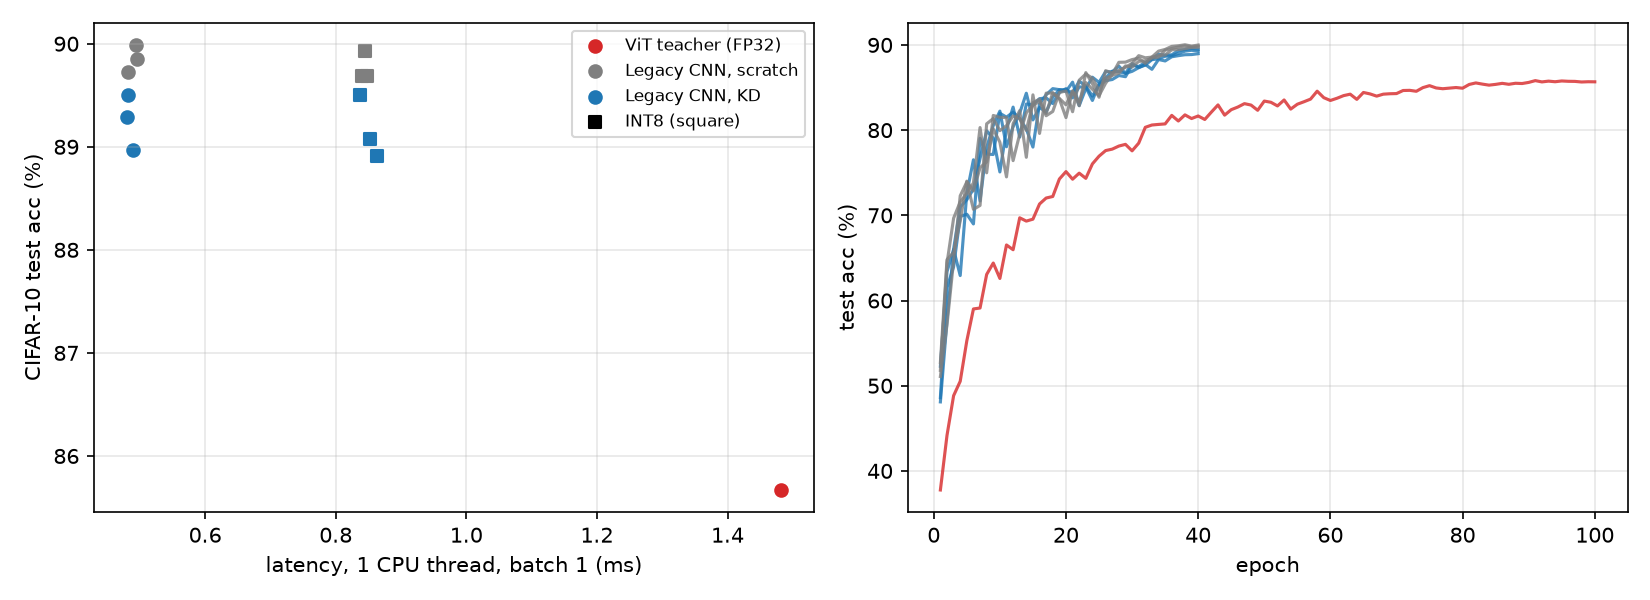
\includegraphics[width=\linewidth]{../results/kd_legacy.png}
\caption{Left: accuracy vs.\ 1-thread batch-1 latency (circles FP32, squares INT8). Right: test accuracy per epoch
(red teacher, gray scratch students, blue KD students).}
\end{figure}

\subsection{Findings}
\begin{enumerate}[label=F\arabic*.]
  \item \textbf{(Q1) The op-set restriction is cheap here.} The legacy student uses no unsupported operator,
        is $11\times$ smaller and $3.0\times$ faster (1 thread, FP32) than the teacher, and is \emph{more} accurate (+4.2 pt).
  \item \textbf{(Q2) Logit KD did not improve compatibility; it transferred the teacher's errors.}
        Overall agreement is unchanged (83.70 vs.\ 83.63). The decomposition shows why: KD raises agreement on the
        teacher's \emph{mistakes} (20.45\% $\rightarrow$ 22.56\%, $\approx$5 pooled std) while slightly lowering it on the teacher's
        correct predictions, so accuracy drops by 0.6 pt. Soft labels from a weaker, architecturally different teacher
        mainly carry its error modes.
  \item \textbf{(Q3) INT8 PTQ preserves accuracy and agreement} ($\le$0.1 pt change) and cuts size $3.9\times$.
        However, \textbf{INT8 was slower than FP32 on this CPU} (0.84 vs.\ 0.49 ms): Apple Silicon's FP32 path is highly
        optimized and qnnpack is not tuned for it. INT8 speed-ups are hardware-dependent, which is exactly why the target
        hardware should be part of the distillation objective.
\end{enumerate}

\section{Limitations and Validity}
\begin{itemize}
  \item \textbf{Weak teacher.} A from-scratch ViT on CIFAR-10 is below the CNN student; the realistic
        backward-compatibility setting (a stronger new model) is not covered. F2 may not hold with a stronger teacher.
  \item \textbf{Emulated hardware.} The op whitelist and 1-thread M4 latency are proxies, not measurements on a real legacy NPU/DSP.
  \item \textbf{Small scale.} One dataset, one student, one KD recipe ($T=4$, $\alpha=0.9$, not tuned), 3 seeds; one teacher run.
  \item \textbf{Augmentation detail.} Batch-shared crop offset (\S2); identical across groups, so comparisons remain controlled.
\end{itemize}

\section{Planned Next Experiments}
\begin{center}\begin{tabular}{p{0.6cm}p{5.0cm}p{8.0cm}}\toprule
Prio & Experiment & Purpose\\\midrule
P0 & Stronger teacher (pre-trained ViT fine-tuned) & Test whether F2 is an artifact of the weak teacher\\
P0 & KD sweep ($T\in\{1,2,4,8\}$, $\alpha$) & Separate ``KD fails'' from ``KD untuned''\\
P1 & Feature / attention-map distillation & Transfer intermediate representations across the attention$\rightarrow$conv gap\\
P1 & Correctness-gated / agreement-targeted loss & Match the teacher where it is right; do not copy its errors (motivated by F2)\\
P2 & Real legacy target (e.g.\ Raspberry Pi, older mobile NPU) & Replace the emulated latency with measured latency; hardware-aware student search\\\bottomrule
\end{tabular}\end{center}

\section{Reproduction Notes}\label{sec:repro}
\texttt{PY=.venv/bin/python ./run\_all.sh} (teacher 36.9 min; scratch student $\approx$2 min, KD student $\approx$5.7 min each, on MPS),
then \texttt{python analyze.py} for \S6.2. Raw per-epoch logs: \texttt{results/*.json}; benchmark: \texttt{results/bench.json};
decomposition: \texttt{results/agreement\_breakdown.json}. PyTorch 2.14, torchvision 0.29, macOS, Apple M4 Max.

\section{Where the Conclusion Stands}
Established: on an emulated legacy target, a conv-only INT8 student can replace a ViT at lower cost with no accuracy loss,
and vanilla logit KD across the attention$\rightarrow$conv gap does not improve behavioural compatibility; instead, it measurably
increases agreement on the teacher's errors. Not established: whether this holds for strong teachers, other KD objectives,
or real legacy hardware; these are the P0--P2 experiments above.

\end{document}
